\section{Introduction}
Artist identification is traditionally performed by \textit{art historians} and \textit{curators} who have expertise and familiarity with different artists and styles of art. This is a complex and interesting problem for computers because identifying an artist does not just require object or face detection; artists can paint a wide variety of objects and scenes. Additionally, many artists from the same time period will have similar styles, and some such as \textbf{Pablo Picasso} (see figure \ref{fig:picasso}) have painted in multiple styles and changed their style over time.

\begin{figure}[H]
	\centering
	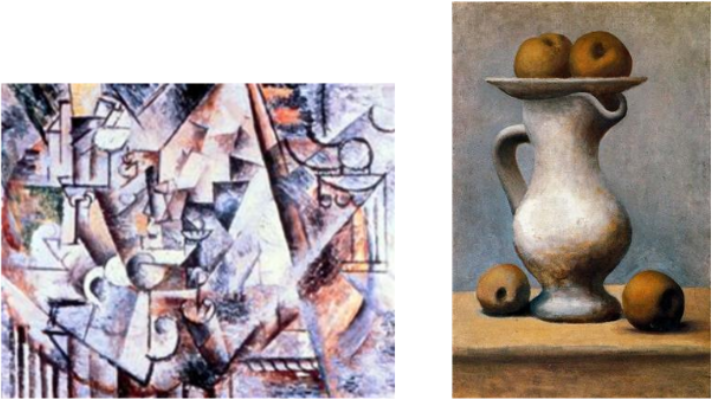
\includegraphics[width=0.4\textwidth]{img/picasso.png}
	\caption{Both of these paintings were created by Pablo Picasso, but they have vastly different styles and content since they correspond to two different periods.}
	\label{fig:picasso}
\end{figure}

\noindent The aim of this project is to use Convolutional Neural Networks for the identification of an artist given a painting. In particular, the CNN networks will be modeled using multiple techniques: from scratch; via pretrained network; networks based on comparison with baseline input and using an ensemble network made of by the best classifiers found.


\subsection{State of the Art}
As mentioned, artist identification has primarily been tackled by humans. An example of that is the Artsy's Art Genome Project \footnote{https://www.artsy.net/categories}, which is led by experts who manually classify art. This strategy is not very scalable even if it is highly precise in the classification (the site is a marketplace of fine-arts for collects, you can find Pisarro, Bansky and other famous artists).

Most prior attempts to apply machine learning to this problem have been feature-based, aiming to identify what qualities most effectively distinguish artists and styles. Many generic image features have been used, including scale-invariant feature transforms (SIFT), histograms of oriented gradients (HOG), and more, but with the focus on discriminating different style in Fine-Art Painting\footnote{T. E. Lombardi. The classification of style in fine-art paint-
ing. ETD Collection for Pace University, 2005}.

The first time the problem of artist identification was really tackled was with J. Jou and S. Agrawal\footnote{J. Jou and S. Agrawal. Artist identification for renaissance paintings.} in 2011, they applied several multi-class classification techniques like Naïve Bayes, Linear Discriminant Analysis, Logistic Regression, K-Means and SVMs and achieve a maximum classification accuracy of 65\% for an unknown painting across 5 artists. 
Later on, the problem of identifying artists was retackled by the \textit{Rijksmuseum Challenge}\footnote{T. Mensink and J. van Gemert. The rijksmuseum challenge: Museum-centered visual recognition. 2014}. The objective of the challenge was to predict the artist, type, material and creation year of the 112,039 photographic reproductions of the artworks exhibited in the Rijksmuseum in Amsterdam (the Netherlands). The year later, Saleh and Elgammal's paper\footnote{B. Saleh and A. M. Elgammal. Large-scale classification of fine-art paintings: Learning the right metric on the right
feature. CoRR, abs/1505.00855, 2015} was the first attempt to identify artists with a large and varied dataset, but still using generic features.

More recent attempts are related to the \textit{Painter by Numbers}, a \textbf{Playground Prediction Competition} by \textit{Kaggle}. This competition used a pairwise comparison scheme: participants had to create an algorithm which needs to examine two images and predict whether the two images are by the same artist or not. Thus, it is not our same objective, however it can be consider the first application of Deep Learning to the problem. The real deal was taken by Nitin Viswanathan\footnote{Nitin Viswanathan, Artist Identification with Convolutional Neural Networks} in 2017.
Viswanathan, using the same dataset of the mentioned \textit{Kaggle Challenge}, proposed the use of ResNet with transfer learning (he first held the weights of the base ResNet constant and updated only the fully-connected layer for a few epochs). This trained network reached a train accuracy of 0.973 and a test accuracy of 0.898.



\subsection{Dataset}